\documentclass{beamer}

\usepackage{listings}
% Copyright 2017 Sergei Tikhomirov, MIT License
% https://github.com/s-tikhomirov/solidity-latex-highlighting/

\usepackage{listings, xcolor}

\definecolor{verylightgray}{rgb}{.97,.97,.97}

\lstdefinelanguage{Solidity}{
	keywords=[1]{anonymous, assembly, assert, balance, break, call, callcode, case, catch, class, constant, continue, constructor, contract, debugger, default, delegatecall, delete, do, else, emit, event, experimental, export, external, false, finally, for, function, gas, if, implements, import, in, indexed, instanceof, interface, internal, is, length, library, log0, log1, log2, log3, log4, memory, modifier, new, payable, pragma, private, protected, public, pure, push, require, return, returns, revert, selfdestruct, send, solidity, storage, struct, suicide, super, switch, then, this, throw, transfer, true, try, typeof, using, value, view, while, with, addmod, ecrecover, keccak256, mulmod, ripemd160, sha256, sha3}, % generic keywords including crypto operations
	keywordstyle=[1]\color{blue}\bfseries,
	keywords=[2]{address, bool, byte, bytes, bytes1, bytes2, bytes3, bytes4, bytes5, bytes6, bytes7, bytes8, bytes9, bytes10, bytes11, bytes12, bytes13, bytes14, bytes15, bytes16, bytes17, bytes18, bytes19, bytes20, bytes21, bytes22, bytes23, bytes24, bytes25, bytes26, bytes27, bytes28, bytes29, bytes30, bytes31, bytes32, enum, int, int8, int16, int24, int32, int40, int48, int56, int64, int72, int80, int88, int96, int104, int112, int120, int128, int136, int144, int152, int160, int168, int176, int184, int192, int200, int208, int216, int224, int232, int240, int248, int256, mapping, string, uint, uint8, uint16, uint24, uint32, uint40, uint48, uint56, uint64, uint72, uint80, uint88, uint96, uint104, uint112, uint120, uint128, uint136, uint144, uint152, uint160, uint168, uint176, uint184, uint192, uint200, uint208, uint216, uint224, uint232, uint240, uint248, uint256, var, void, ether, finney, szabo, wei, days, hours, minutes, seconds, weeks, years},	% types; money and time units
	keywordstyle=[2]\color{teal}\bfseries,
	keywords=[3]{block, blockhash, coinbase, difficulty, gaslimit, number, timestamp, msg, data, gas, sender, sig, value, now, tx, gasprice, origin},	% environment variables
	keywordstyle=[3]\color{violet}\bfseries,
	identifierstyle=\color{black},
	sensitive=false,
	comment=[l]{//},
	morecomment=[s]{/*}{*/},
	commentstyle=\color{gray}\ttfamily,
	stringstyle=\color{red}\ttfamily,
	morestring=[b]',
	morestring=[b]"
}

\lstset{
  language=Solidity,
  escapeinside={<@}{@>},
	backgroundcolor=\color{verylightgray},
	extendedchars=true,
	basicstyle=\footnotesize\ttfamily,
	showstringspaces=false,
	showspaces=false,
	numbers=left,
	numberstyle=\footnotesize,
	numbersep=9pt,
	tabsize=2,
	breaklines=true,
	showtabs=false,
	captionpos=b
}


\usecolortheme{beaver}

\AtBeginSection
{
  \begin{frame}
    \frametitle{Table of Contents}
    \tableofcontents[currentsection]
  \end{frame}
}

\setbeamertemplate{itemize items}{\textbullet}
\setbeamertemplate{footline}[text line]{%
  \parbox{\linewidth}{\vspace*{-8pt}
    \insertshorttitle\hfill\insertshortauthor\hfill\insertframenumber
  }
}
\setbeamertemplate{navigation symbols}{}

\begin{document}

\title{Formal Verification in Scala}
% \subtitle{The Decentralized Autonomous Organization}
\author{Ramon Boss, Anna Doukmak}

\frame{\titlepage}

\begin{frame}
  \frametitle{Table of Contents}
  \tableofcontents
\end{frame}

%%%%%%%%%%%%%%%%%%%%%%%%%%%%%%%%%%%%%%%%%%%%%%%%%%%%%%%%%%%%%%%%%%%%%%%%%%%%%%%%
\section{What is The DAO}
%%%%%%%%%%%%%%%%%%%%%%%%%%%%%%%%%%%%%%%%%%%%%%%%%%%%%%%%%%%%%%%%%%%%%%%%%%%%%%%%

\begin{frame}
\frametitle{What is The DAO}
\begin{columns}
  \begin{column}{0.5\textwidth}
  Basics
  \begin{itemize}
    \item Investment fund
    \item Autonomous
    \item Voting right based on invested amount
  \end{itemize}
  \end{column}
  \pause
  \begin{column}{0.5\textwidth}
    Technology
    \begin{itemize}
      \item An open-source software
      \item Written in Solidity
      \item Build on Ethereum blockchain
    \end{itemize}
  \end{column}
\end{columns}
\end{frame}


\begin{frame}[fragile]
\frametitle{Initial Phase}
\begin{itemize}
  \item Defines the contract
  \item Minimum ETH needed
  \item Fixed end time
\end{itemize}
\pause
\begin{lstlisting}[language=Solidity]
contract DAO is DAOInterface {
  uint constant minProposalDebatePeriod = 2 weeks;
  uint public proposalDeposit;
  mapping (address => bool) public allowedRecipients;

  function DAO(uint _proposalDeposit) {
    proposalDeposit = _proposalDeposit;
    allowedRecipients[address(this)] = true;
  }
}
\end{lstlisting}
\end{frame}


\begin{frame}
\frametitle{Investors}
\begin{itemize}
  \item Invest in The DAO
  \item A Ethereum wallet address
  \item Gets DAO tokens
  \item Receive reward
\end{itemize}
\end{frame}


\begin{frame}
\frametitle{Example Investors}
\centering
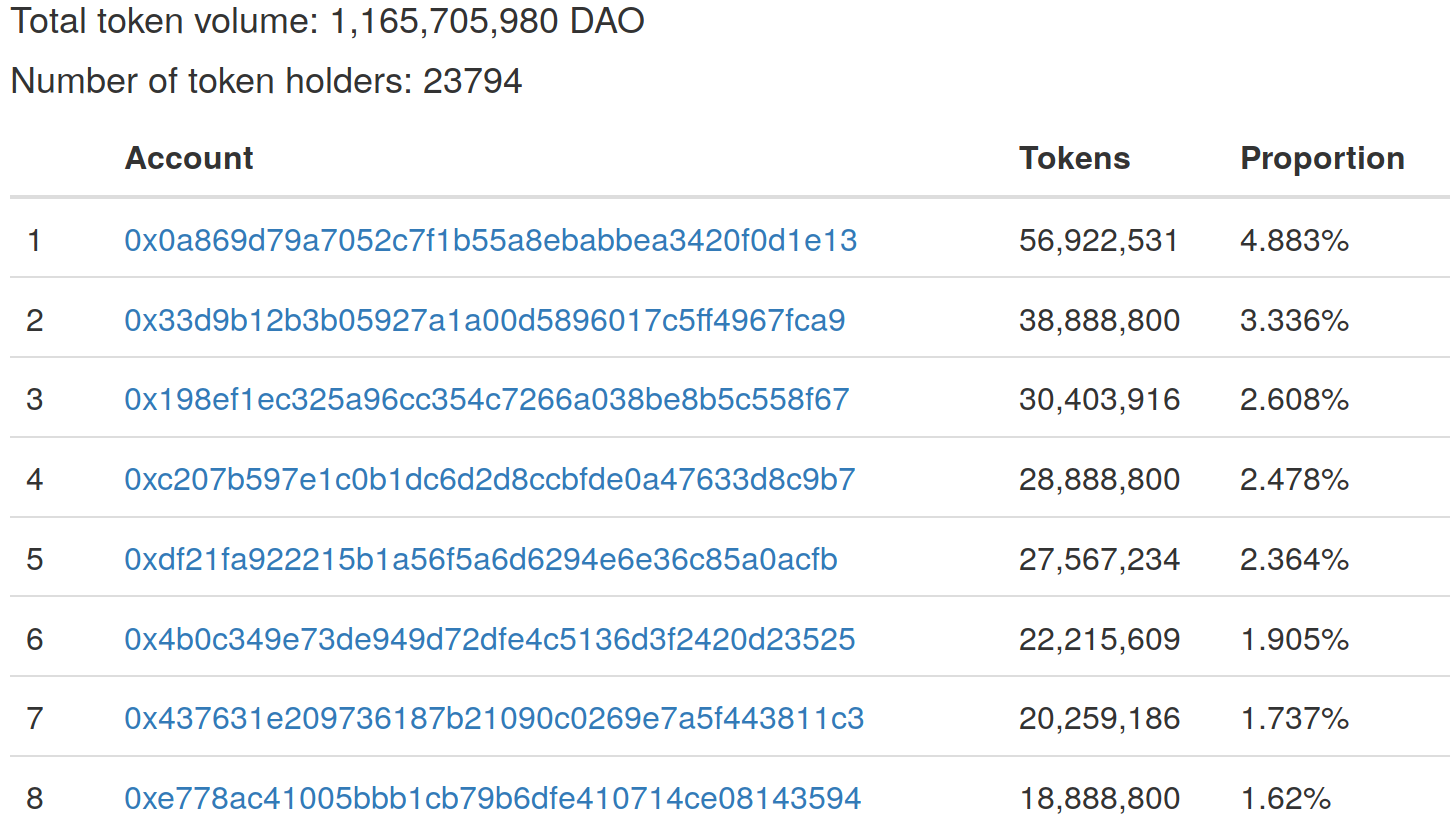
\includegraphics[width=\textwidth,height=0.8\textheight,keepaspectratio]{assets/token_holders.png}
\end{frame}


\begin{frame}[fragile]
\frametitle{Proposal}
\begin{itemize}[<1-2>]
  \item Recipient
  \item Amount
  \item Deadline
  \item Creator
\end{itemize}
\pause
\begin{lstlisting}[language=Solidity]
struct Proposal {
  address recipient;
  uint amount;
  string description;
  uint votingDeadline;
  uint proposalDeposit;
  address creator;
}
\end{lstlisting}
\end{frame}


\begin{frame}
\frametitle{Example Proposal}
Mobotiq's vision of modular Electric Vehicles that can be rented P2P is a perfect fit for the blockchain. Integration with Ethereum could enable the development of fully autonomous, self-renting vehicles.
\end{frame}


\begin{frame}
\frametitle{Proposal List}
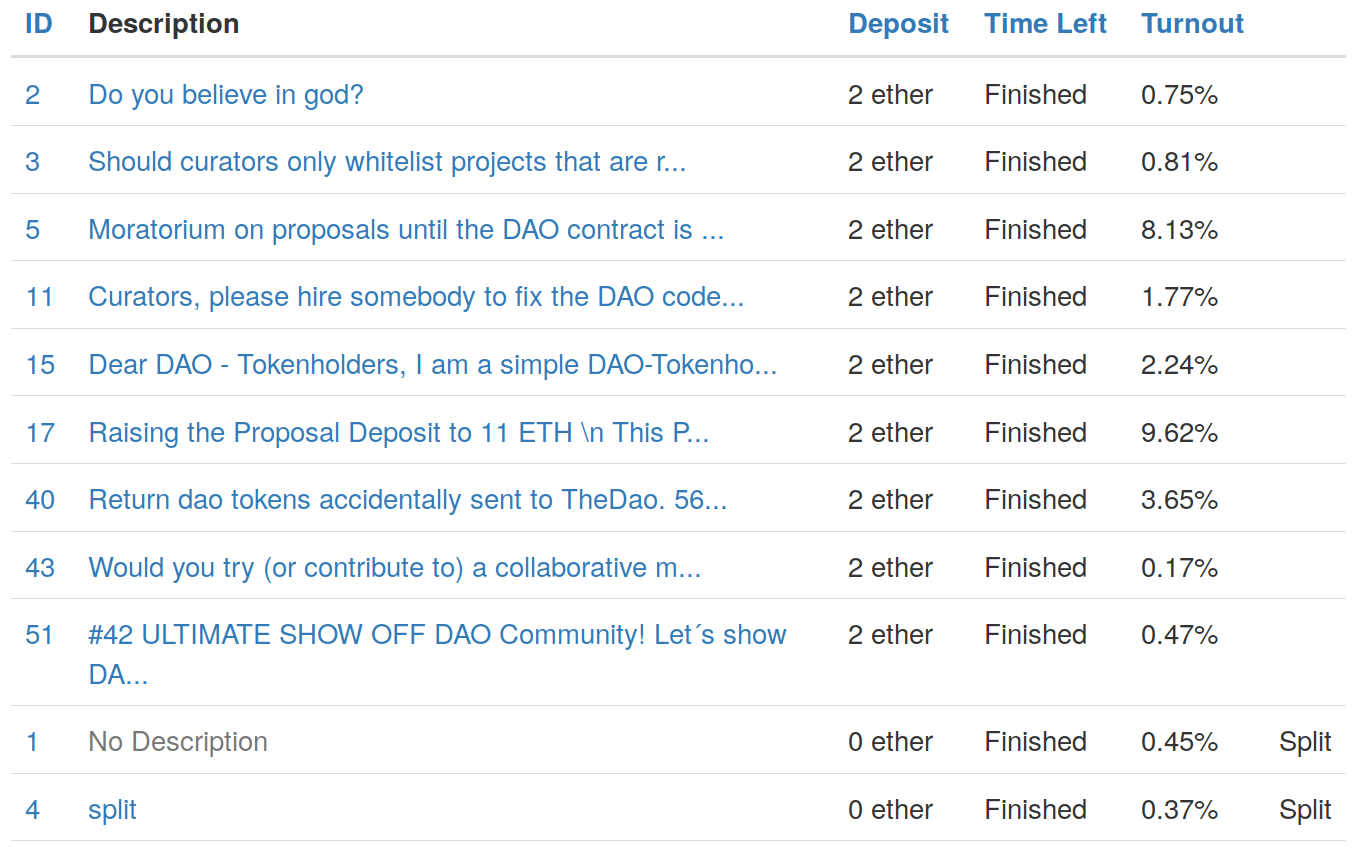
\includegraphics[width=\textwidth,height=0.8\textheight,keepaspectratio]{assets/proposals.png}
\end{frame}

%%%%%%%%%%%%%%%%%%%%%%%%%%%%%%%%%%%%%%%%%%%%%%%%%%%%%%%%%%%%%%%%%%%%%%%%%%%%%%%%
\section{Majority voting attack}
%%%%%%%%%%%%%%%%%%%%%%%%%%%%%%%%%%%%%%%%%%%%%%%%%%%%%%%%%%%%%%%%%%%%%%%%%%%%%%%%

\begin{frame}
\frametitle{Curator}
\begin{itemize}
  \item Controls the whitelist
  \item Checks proposals
\end{itemize}
\end{frame}

%%%%%%%%%%%%%%%%%%%%%%%%%%%%%%%%%%%%%%%%%%%%%%%%%%%%%%%%%%%%%%%%%%%%%%%%%%%%%%%%
\section{Why there is no new The DAO}
%%%%%%%%%%%%%%%%%%%%%%%%%%%%%%%%%%%%%%%%%%%%%%%%%%%%%%%%%%%%%%%%%%%%%%%%%%%%%%%%

\begin{frame}
\frametitle{Why there is no new The DAO}
\begin{itemize}
	\item Profitableness
	\item Law
	\item Voting problem
	\item The stalker
\end{itemize}
\end{frame}


\end{document}
